% Con correcciones de Mollerach

\section{Acerca de la tesis de licenciatura}

En el trabajo de tesis de licenciatura se analizaron los efectos de las variaciones de los parámetros del clima sobre el desarrollo en la atmósfera de las lluvias atmosféricas. Se analizaron datos del arreglo de detectores espaciados 1500 m entre sí, conocido como \emph{arreglo principal}, del Observatorio Pierre Auger en el periodo 2005-2018,  extendiendo  así los periodos de tiempo estudiados anteriormente en los siguientes trabajos \cite{abraham2009atmospheric}, \cite{abreu2012description}   y \cite{aab2017impact} . Se emuló los resultados de la corrección de la modulación del clima sobre el periodo 2005-2015 de la colaboración Pierre Auger \cite{aab2017impact}, obteniéndose resultados compatibles. Se observó que posterior a la corrección, la modulación del clima se vio disminuida. Para eventos con energía mayor a $2\,$EeV, esta modulación es despreciable.

En el mismo trabajo, se estudió la modulación del clima mediante el valor del $S_{38}$ sin la corrección propuesta por trabajos anteriores. Se observó que los parámetros del clima obtenidos de estos datos son compatibles con los utilizados en la reconstrucción oficial. Se realizó una corrección de los efectos atmosféricos a la energía con estos coeficientes, observándose que la modulación era despreciable para energías mayores a $2\,$EeV al igual que la reconstrucción oficial. 

\section{Acerca del archivo con todos los disparos}

El análisis anterior fue realizado sobre los eventos medidos por el arreglo principal utilizando el disparo estándar. Este disparo tiene una eficiencia completa para eventos de energía mayor a $2.5\,$EeV. Por lo que el análisis de anisotropías en el rango de energía entre $1\,$EeV - $2\,$EeV, requiere factores relacionados a la eficiencia función de la energía que se obteniendo de manera fenomenológica \cite{taborda}.

Para superar esta dificultad,  a partir del año 2013 se implementó otros protocolos de disparo en el arreglo principal, llamados Mops y ToTs. Con esta mejora, la eficiencia completa se alcanza para una energía mayor a $1\,$EeV. De esta manera se aumenta la cantidad de eventos a estudiar en el rango $1\,$EeV - $2\,$EeV y no son necesarios factores relacionados a la eficiencia. La desventaja es que el disparo estándar tiene una mayor cantidad de datos ya que se adquieren datos  desde el año 2004 con ese protocolo.

\section{Acerca de los eventos} \label{filtro}

Para poder prescindir de los factores de corrección a los datos de los eventos, se aplican cortes a los datos para asegurar la eficiencia completa de los detectores. Por eso se implementan  límites en ángulo cenital, en la cantidad de vecinos al tanque de mayor señal, además de restringirse a los datos fueron medidos en condiciones normales, es decir cuando los sistemas de comunicación del Observatorio funciona sin incovenientes.

%  Esto da como resultado límites superiores
% al ángulo cenital θ max y umbrales de energía para los cuales se satisface la condición de
% eciencia. En Auger por ejemplo, el SD principal tiene eciencia de 100 % para energías
% arriba de 3 EeV para θ max = 60 ◦ o arriba de 4 EeV para θ max = 80 ◦ .

A partir de los registros de eventos del arreglo principal con todos los disparos, se consideran solamente los eventos que cumplan las siguientes características:

    \begin{enumerate}
      \item Ángulo cenital $\theta < 60^o$
      \item $ib=1$ \emph{Bad period flag}. Un valor de 1 indica un buen periodo en el cual los datos son recopilados sin inconvenientes.
      \item Buena reconstrucción de la lluvia atmósferica asociada al evento
      \item La cantidad de vecinos alrededor del tanque con mayor señal sea de 6 tanques.
    \end{enumerate}
   
\section{Cálculo de los coeficientes de Fourier para el análisis de anisotropía en ascensión recta}

  \subsection{Variaciones relativas de los hexágonos} \label{peso_hexagonos}

    Los pesos de los eventos son importantes para el cálculo de anisotropías, ya que las mismas son pequeñas y eliminar todo factor espúreo en el análisis es importante. Para una representación fiel entre los registros de los hexágonos y los pesos de los eventos, se optó por utilizar $288$ segmentos ya que si consideramos para $24$ hrs del día, cada segmento tiene un ancho de $5$\, min. Esto es conveniente ya que la actualización tanto del clima como de los hexágonos se realiza una vez cada $5$\,min.

      %\begin{enumerate}[itemindent=0cm,labelsep=0cm]
        %\item 
        Se establecen una frecuencia a estudiar $f$ y el rango de tiempo de análisis, por ejemplo la frecuencia solar $f_{Solar}= 365.25\,$ ciclos en un año entre los años 2013 y 2020. Existe un registro del Observatorio de los hexágonos 6T5 que se actualiza cada 5 min. Cada dato tomado durante el rango seleccionado, se clasifica según la cantidad de horas $t$ desde un momento de referencia $t_0$. Esta referencia $t_0$ es el 1 de Enero del 2004 a las $00:00:00\,$GMT, o  $21$ hrs del 31 de Diciembre del 2003, según la hora local de Malargüe.

        %\item
        Podemos asociar una coordenada angular $h$   a $t$  y $f$  utilizando la siguiente expresión
         \begin{equation}
          h = t \times \frac{360}{24} \times\frac{f}{f_{Solar}} + h_0
          \label{eq:h_horas} 
        \end{equation}
        El factor $\nicefrac{f}{f_{Solar}}$ sirve para hacer un escaleo de las horas entre diferentes frecuencias. Se usa como referencia la $f_{Solar}$ dado que las horas (solares) se basan en esta frecuencia, y el valor de $h_0=31.4971$ representa la ascensión recta del cenit en el momento utilizado como referencia.
        
        %\item 
        Para simplificar el cálculo del peso de los hexágonos, se divide los 360$^o$ de la ascensión recta en $L$ segmentos de $\nicefrac{360}{L}$ hrs cada uno. Para clasificar un dato se  toma  el valor $h$  y se calcula
        \begin{equation}
          h' = h\, mod \,360 
          \label{eq:h_primado}
        \end{equation}
        donde la función $mod$ representa la función módulo. Luego con el valor de $h'$ se asigna al dato con el segmento $k$ correspondiente.
        \begin{equation}
          k = \bigg \lceil \frac{h'}{360}\times L \bigg \rceil
        \end{equation}
        done $\lceil a \rceil$ representa la función techo \footnote{La función techo da como resultado el número entero más próximo por exceso}. Por ejemplo, si optamos por $L=24$ y un registro en particular resulta con  $h=395\,^o$, esto implica que $h'= 35\,$hr y $k=\lceil 2.3 \rceil=3$, por lo tanto, este registro corresponde al segmento en la $3^{a}$ posición.

        %\item
        Una vez clasificado todos los datos del registro de hexágonos, se calcula la suma  $N_{hex, j}$ de los registros de hexágonos que cayeron un segmento $j$ dado. Para definir la variación relativa de hexágonos  $\Delta N_{cell,k}$ de un segmento $k$ en particular, se necesita la media de hexágonos por segmento:
       
       \begin{align}
         \langle N \rangle &= \sum^{L}_{i=1} \frac{N_{hex, i}}{L}  \qquad
         \Delta N_{cell,k} = \frac{N_{cell, k}}{\langle N \rangle}  \label{epepe}
       \end{align}

      En la Fig.\ref{fig:pesos_referencia} se muestran las variaciones relativas de los hexágonos en función de la ascensión recta del cenit del observatorio para las frecuencias sidérea, solar y antisidérea. Este análisis fue realizado en el marco del trabajo \cite{referencia_pesos} en el periodo 2004-2017. 

          \begin{figure}[H]
          \centering
              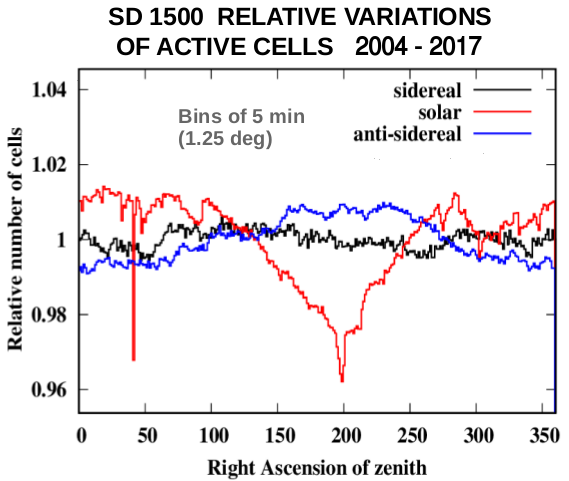
\includegraphics[width=0.8\linewidth]{pesos_referencia.png}  
              \caption{Valores de $\Delta N_{cell, k}$ en el rango 2004-2017 para distintas frecuencias obtenidas en el trabajo \cite{referencia_pesos}.}
              \label{fig:pesos_referencia}
        \end{figure}

       En la Fig.\ref{fig:pesos_ejemplo} se observa valores obtenidos de $\Delta N_{cell,k}$ en función de la ascensión recta del cenit  para $L=288$ segmentos con el programa escrito para este informe, utilizando el mismo conjunto de datos que el utilizado para obtener los resultados la Fig.\ref{fig:pesos_referencia} desde el 1 de Enero del 2004 a las $00:00:00\,$hrs GMT  hasta el 1 de Enero del 2017 a las $00:00:00\,$hrs GMT. Se  observa que estos los resultados obtenidos son compatibles con la Fig.\ref{fig:pesos_referencia}
 

       \begin{figure}[H]
          \centering
              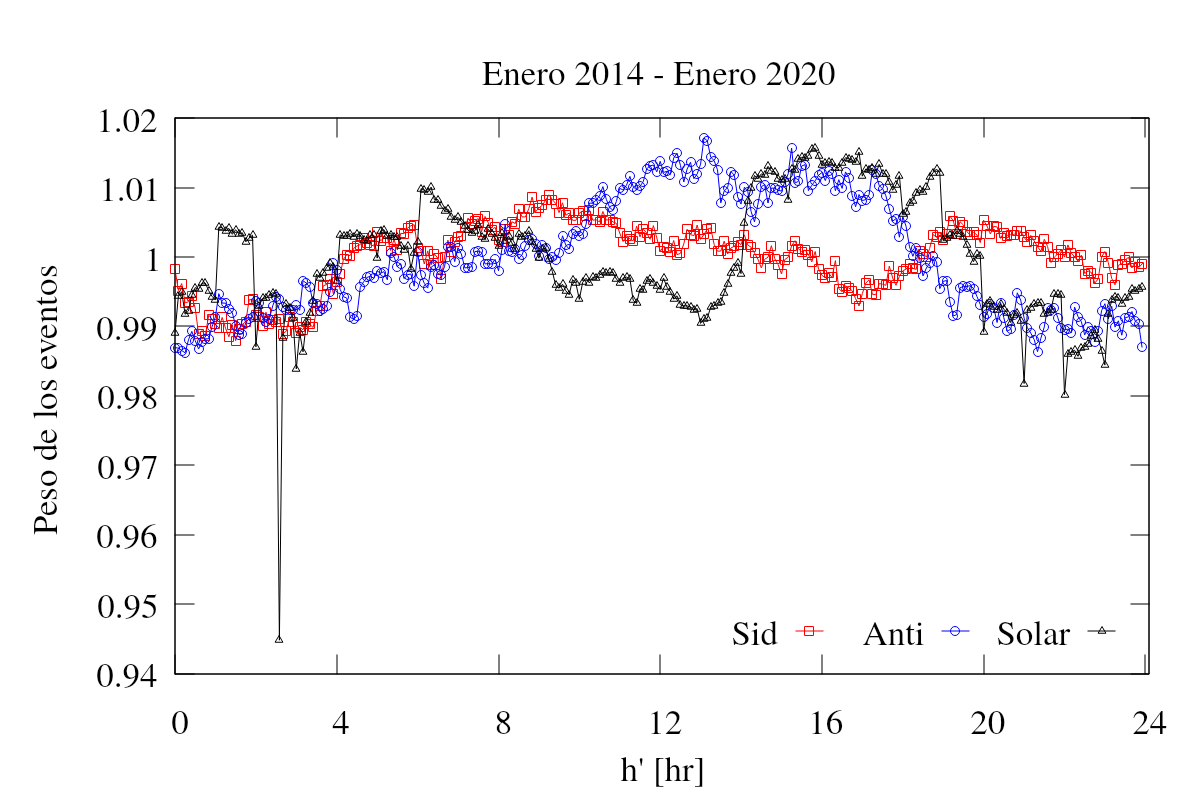
\includegraphics[width=0.8\linewidth]{weigths_2020.png}
              \caption{Valores de $\Delta N_{cell, k}$ en el rango 2004-2017 para distintas frecuencias utilizando el código escrito en este trabajo.}
              \label{fig:pesos_ejemplo}
        \end{figure}


%%%%%%%%%%%%%%%%%%%%%%%%%%%%%%%%%%%%%%%%%%%%%%%%%%%%%%%%%%%%%%%%%%%%%%%%%%%%%%%%%%%%%%%%%%%%%%%%%%%%%%%%%%%%%%%%%%%%%%%%%%%%%%%%%%%%%%%%%%%%%%%%%%%%%%%%%%%%%%%%%%%%%%%%%%%%%%%%%%%%%%%%%%%%%%%%%%%%%%%%%%%%%%%%%%%%%%%%%%%%%%%%%%%%%%%%

  \subsection{Cálculo de Rayleigh para una frecuencia dada} \label{rayleigh}

        \begin{enumerate}
        \item Fijando un rango de tiempo y un rango de energía en el cual se desea estudiar la anisotropía, se establece una frecuencia en particular $f$ a analizar.

        \item Con los eventos ya filtrados según el criterio de la sección \ref{filtro}, asigno cada evento $i$ un valor $h_i$, definida en la Ec.\ref{eq:h_horas}

        \item Para asignar el peso correspondiente al evento, se asocia a un segmento $k$, calculado en la sección \ref{peso_hexagonos}, mediante el valor de $h'_i$ definido en la Ec.\,\ref{eq:h_primado}. Luego, el peso asignado $w_i$  al evento $i$ es
        \begin{equation*}
           w_{i}= (\Delta N_{cell,k})^{-1}
        \end{equation*} 
         
        \item Para el análisis en frecuencias, a partir del valor de $h_i$ se asigna un ángulo $\tilde{\alpha}_i$ como:
        \begin{equation}
         \tilde{\alpha}_i = 2\pi \frac{h}{24} + \alpha_i -\alpha_{cenit,i}
        \end{equation}
        donde $\alpha_i$  representa la ascensión recta del evento y $\alpha_{cenit,i}$ la ascensión recta en el cenit del observatorio en el momento del evento. A partir de este ángulo $\tilde{\alpha}_i$ se realiza en análisis en frecuencias.

        \item Para calcular los coeficientes de Fourier del primer armónico $a$ y $b$, se siguen los siguiente pasos:
        \begin{enumerate}
          \item Por cada evento  $i$ se calculan los siguientes valores:
          \begin{align}
             a_i' = {w_i}\cos\tilde{\alpha}_i \qquad
             b_i' = {w_i}\sin\tilde{\alpha}_i
         \end{align}
         \item Una vez que se obtuvieron los valores de $a_i'$ y $b_i'$ para todos los eventos en el rango de tiempo estudiado, se calculan los coeficientes mediante:
         \begin{alignat}{3}
          \mathcal{N} &= \sum^{Eventos}_i w_i \\
            a &= \frac{2}{\mathcal{N}} \sum^{Eventos}_i a_i' \qquad
            b = \frac{2}{\mathcal{N}} \sum^{Eventos}_i b_i'  
         \end{alignat}
        \end{enumerate}
        \item Con los coeficientes es posible calcular la amplitud de la frecuencia estudiada $\tilde{r}$ y la fase $\phi$. Otros parámetros calculados para el análisis son la probabilidad $P(\tilde{r})$ de que la amplitud obtenida sea producto de una variación de ruido, y el valor de amplitud $r_{99}$ para que dicha probabilidad sea del $1$\%. 
        \begin{alignat}{3}
            \tilde{r} &= \sqrt{a^2 +b^2}             
               \qquad &&   \phi&&= \arctan\frac{a}{b}\\
          P(\tilde{r})&= \exp(-\mathcal{N}\frac{\tilde{r}^2}{4}) 
             \qquad &&   r_{99}&&= \sqrt{\frac{-4\log(0.01)}{\mathcal{N}}}
        \end{alignat}

      \end{enumerate}

    Una forma de validar el código para el análisis de anisotropía es comparar los resultados del código con los obtenidos en otros trabajos \cite{taborda}. En la Fig.\ref{fig:sin_pesos_referencia} se muestra el análisis hecho sobre el mismo conjunto de eventos. Estos eventos fueron adquiridos con el disparo estándar desde el 1 de Enero del 2004 a las $00:00:00\,$GMT  hasta el 1 de Enero del 2017 a las $00:00:00\,$GMT. Se consideraron los eventos por encima de $8\,$EeV que además cumplan las condiciones dadas en la sección \ref{filtro}.  En esta figura que los resultados obtenidos en \cite{taborda} y con el código utilizado por este trabajo son indistinguibles. 

      \begin{figure}[H]
        \centering
        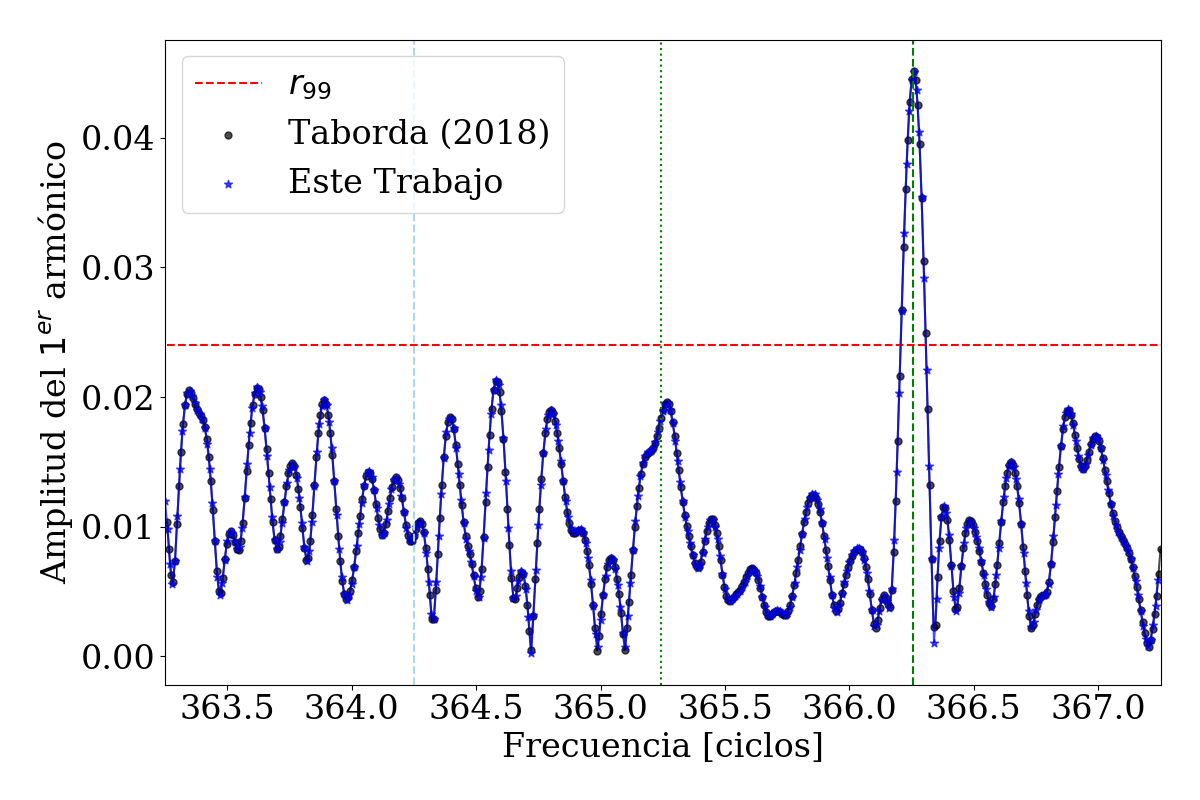
\includegraphics[width=0.75\linewidth]{sin_pesos_referencia_8_EeV.png}
        \caption{Comparación entre los análisis de anisotropía hechos para el mismo conjunto de datos, con el código de \cite{taborda} y con el código escrito para este trabajo.}
        \label{fig:sin_pesos_referencia}
      \end{figure}